\section{Конструкторский раздел}
%В этом разделе будет приведено проектирование базы данных и проектирование приложения.
%Также будет спроектирован триггер, осуществляющие автоматически пересчитывать рейтинга турнира при добавлении новых оценок.
\subsection{Проектирование базы данных}

Выделяются следующие сущности, которые должны хранить в базе данных.

\begin{enumerate}
	\item Users --- таблица пользователей;
	\item Countries --- таблица стран;
	\item Stadiums --- таблица стадионов;
	\item Feedbacks --- таблица отзывов;
	\item Requests --- таблица заявок пользователей;
	\item Leagues --- таблица турниров;
	\item Clubs --- таблица клубов;
	\item Matches --- таблица матчей;
	\item League\_club --- таблица, реализующая связь многие к многим.
\end{enumerate}

На основе диаграммы сущность-связей, приведенной на рисунке \ref{img:ER} определяются стуктуры столбцов, их типы и органичения.

\begin{table}[H]
	\begin{center}
		\caption{Сведение о таблице users}
		\begin{tabular}{|c|c|c|c|}
			\hline
			Столбец & Тип данных & Ограничения & Значение \\
			\hline
			id & serial & PRIMARY KEY & Идентификатор \\
			\hline
			last\_name & VARCHAR(32) & & Фамилия \\
			\hline
			first\_name & VARCHAR(32) & & Имя\\
			\hline
			age & INT &  & Возраст\\
			\hline
			login & VARCHAR(64) & NOT NULL &  Логин \\
			\hline
			password & VARCHAR(64) & NOT NULL & Пароль \\
			\hline
			role & VARCHAR(64) & NOT NULL & Права доступа \\
			\hline
			id\_club & INT &  & ID клуба \\
			\hline			
		\end{tabular}
		\label{table:db:users}
	\end{center}
\end{table}

\begin{table}[H]
	\begin{center}
		\caption{Сведение о таблице leagues}
		\begin{tabular}{|c|c|c|c|}
			\hline
			Столбец & Тип данных & Ограничения & Значение \\
			\hline
			id & SERIAL & PRIMARY KEY & Идентификатор \\
			\hline
			name & VARCHAR(64) & NOT NULL & Название турнира \\
			\hline
			rating & DOUBLE & NOT NULL & Рейтинг турнира\\
			\hline
			id\_user & INT & FOREIGN KEY &  ID пользователя \\
			\hline
			id\_country & INT & FOREIGN KEY & ID страны \\
			\hline
		\end{tabular}
		\label{table:db:league}
	\end{center}
\end{table}

\begin{table}[H]
	\begin{center}
		\caption{Сведение о таблице clubs}
		\begin{tabular}{|c|c|c|c|}
			\hline
			Столбец & Тип данных & Ограничения & Значение \\
			\hline
			id & SERIAL & PRIMARY KEY & Идентификатор \\
			\hline
			name & VARCHAR(64) & NOT NULL & Название команды \\
			\hline
			id\_country & INT & FOREIGN KEY & ID страны \\
			\hline
		\end{tabular}
		\label{table:db:club}
	\end{center}
\end{table}

\begin{table}[H]
	\begin{center}
		\caption{Сведение о таблице stadiums}
		\begin{tabular}{|c|c|c|c|}
			\hline
			Столбец & Тип данных & Ограничения & Значение \\
			\hline
			id & SERIAL & PRIMARY KEY & Идентификатор \\
			\hline
			name & VARCHAR(64) & NOT NULL & Название стадиона \\
			\hline
			capacity & INT & NOT NULL & Количество мест \\
			\hline
			id\_country & INT & FOREIGN KEY & ID страны \\
			\hline
		\end{tabular}
		\label{table:db:stadium}
	\end{center}
\end{table}

\begin{table}[H]
	\begin{center}
		\caption{Сведение о таблице countries}
		\begin{tabular}{|c|c|c|c|}
			\hline
			Столбец & Тип данных & Ограничения & Значение \\
			\hline
			id & SERIAL & PRIMARY KEY & Идентификатор \\
			\hline
			name & VARCHAR(64) & NOT NULL & Название страны \\
			\hline
			continent & VARCHAR(64) & NOT NULL & Континент \\
			\hline
		\end{tabular}
		\label{table:db:country}
	\end{center}
\end{table}

\begin{table}[H]
	\begin{center}
		\caption{Сведение о таблице feedbacks}
		\begin{tabular}{|c|c|c|c|}
			\hline
			Столбец & Тип данных & Ограничения & Значение \\
			\hline
			id & SERIAL & PRIMARY KEY & Идентификатор \\
			\hline
			mark & INT & NOT NULL & Оценка \\
			\hline
			id\_user & INT & FOREIGN KEY & ID пользователя \\
			\hline
			id\_league & INT & FOREIGN KEY & ID турнира \\
			\hline
		\end{tabular}
		\label{table:db:feedback}
	\end{center}
\end{table}

\begin{table}[H]
	\begin{center}
		\caption{Сведение о таблице requests}
		\begin{tabular}{|c|c|c|c|}
			\hline
			Столбец & Тип данных & Ограничения & Значение \\
			\hline
			id & SERIAL & PRIMARY KEY & Идентификатор \\
			\hline
			created\_time & DATE & NOT NULL & Время создания \\
			\hline
			id\_user & INT & FOREIGN KEY & ID пользователя \\
			\hline
			id\_club & INT & FOREIGN KEY & ID клуба \\
			\hline
			id\_league & INT &  & ID турнира \\
			\hline
		\end{tabular}
		\label{table:db:request}
	\end{center}
\end{table}

\begin{table}[H]
	\begin{center}
		\caption{Сведение о таблице matches}
		\begin{tabular}{|c|c|c|c|}
			\hline
			Столбец & Тип данных & Ограничения & Значение \\
			\hline
			id & SERIAL & PRIMARY KEY & Идентификатор \\
			\hline
			goal\_home & DATE &  & Голы домашнего клуба \\
			\hline
			goal\_guest & INT &  & Голы гостевого клуба \\
			\hline
			id\_league & INT & FOREIGN KEY & ID турнира \\
			\hline
			id\_stadium & INT & FOREIGN KEY & ID стадиона \\
			\hline
			id\_home & INT & FOREIGN KEY & ID дом. клуба \\
			\hline
			id\_guest & INT & FOREIGN KEY & ID гост. клуба \\
			\hline
			week & INT & NOT NULL & Неделя \\
			\hline
			time\_start & VARCHAR(64) & NOT NULL & Время проведения матча \\
			\hline						
		\end{tabular}
		\label{table:db:match}
	\end{center}
\end{table}

\begin{table}[H]
	\begin{center}
		\caption{Сведение о таблице leagueclub}
		\begin{tabular}{|c|c|c|c|}
			\hline
			Столбец & Тип данных & Ограничения & Значение \\
			\hline
			id & SERIAL & PRIMARY KEY & Идентификатор \\
			\hline
			id\_league & INT & FOREIGN KEY & ID турнира \\
			\hline
			id\_club & INT & FOREIGN KEY & ID клуба \\
			\hline
		\end{tabular}
		\label{table:db:leagueclub}
	\end{center}
\end{table}

На рисунке \ref{img:ERD} представлена ER-диаграмма базы данных.

\begin{figure}[h]
	\centering
	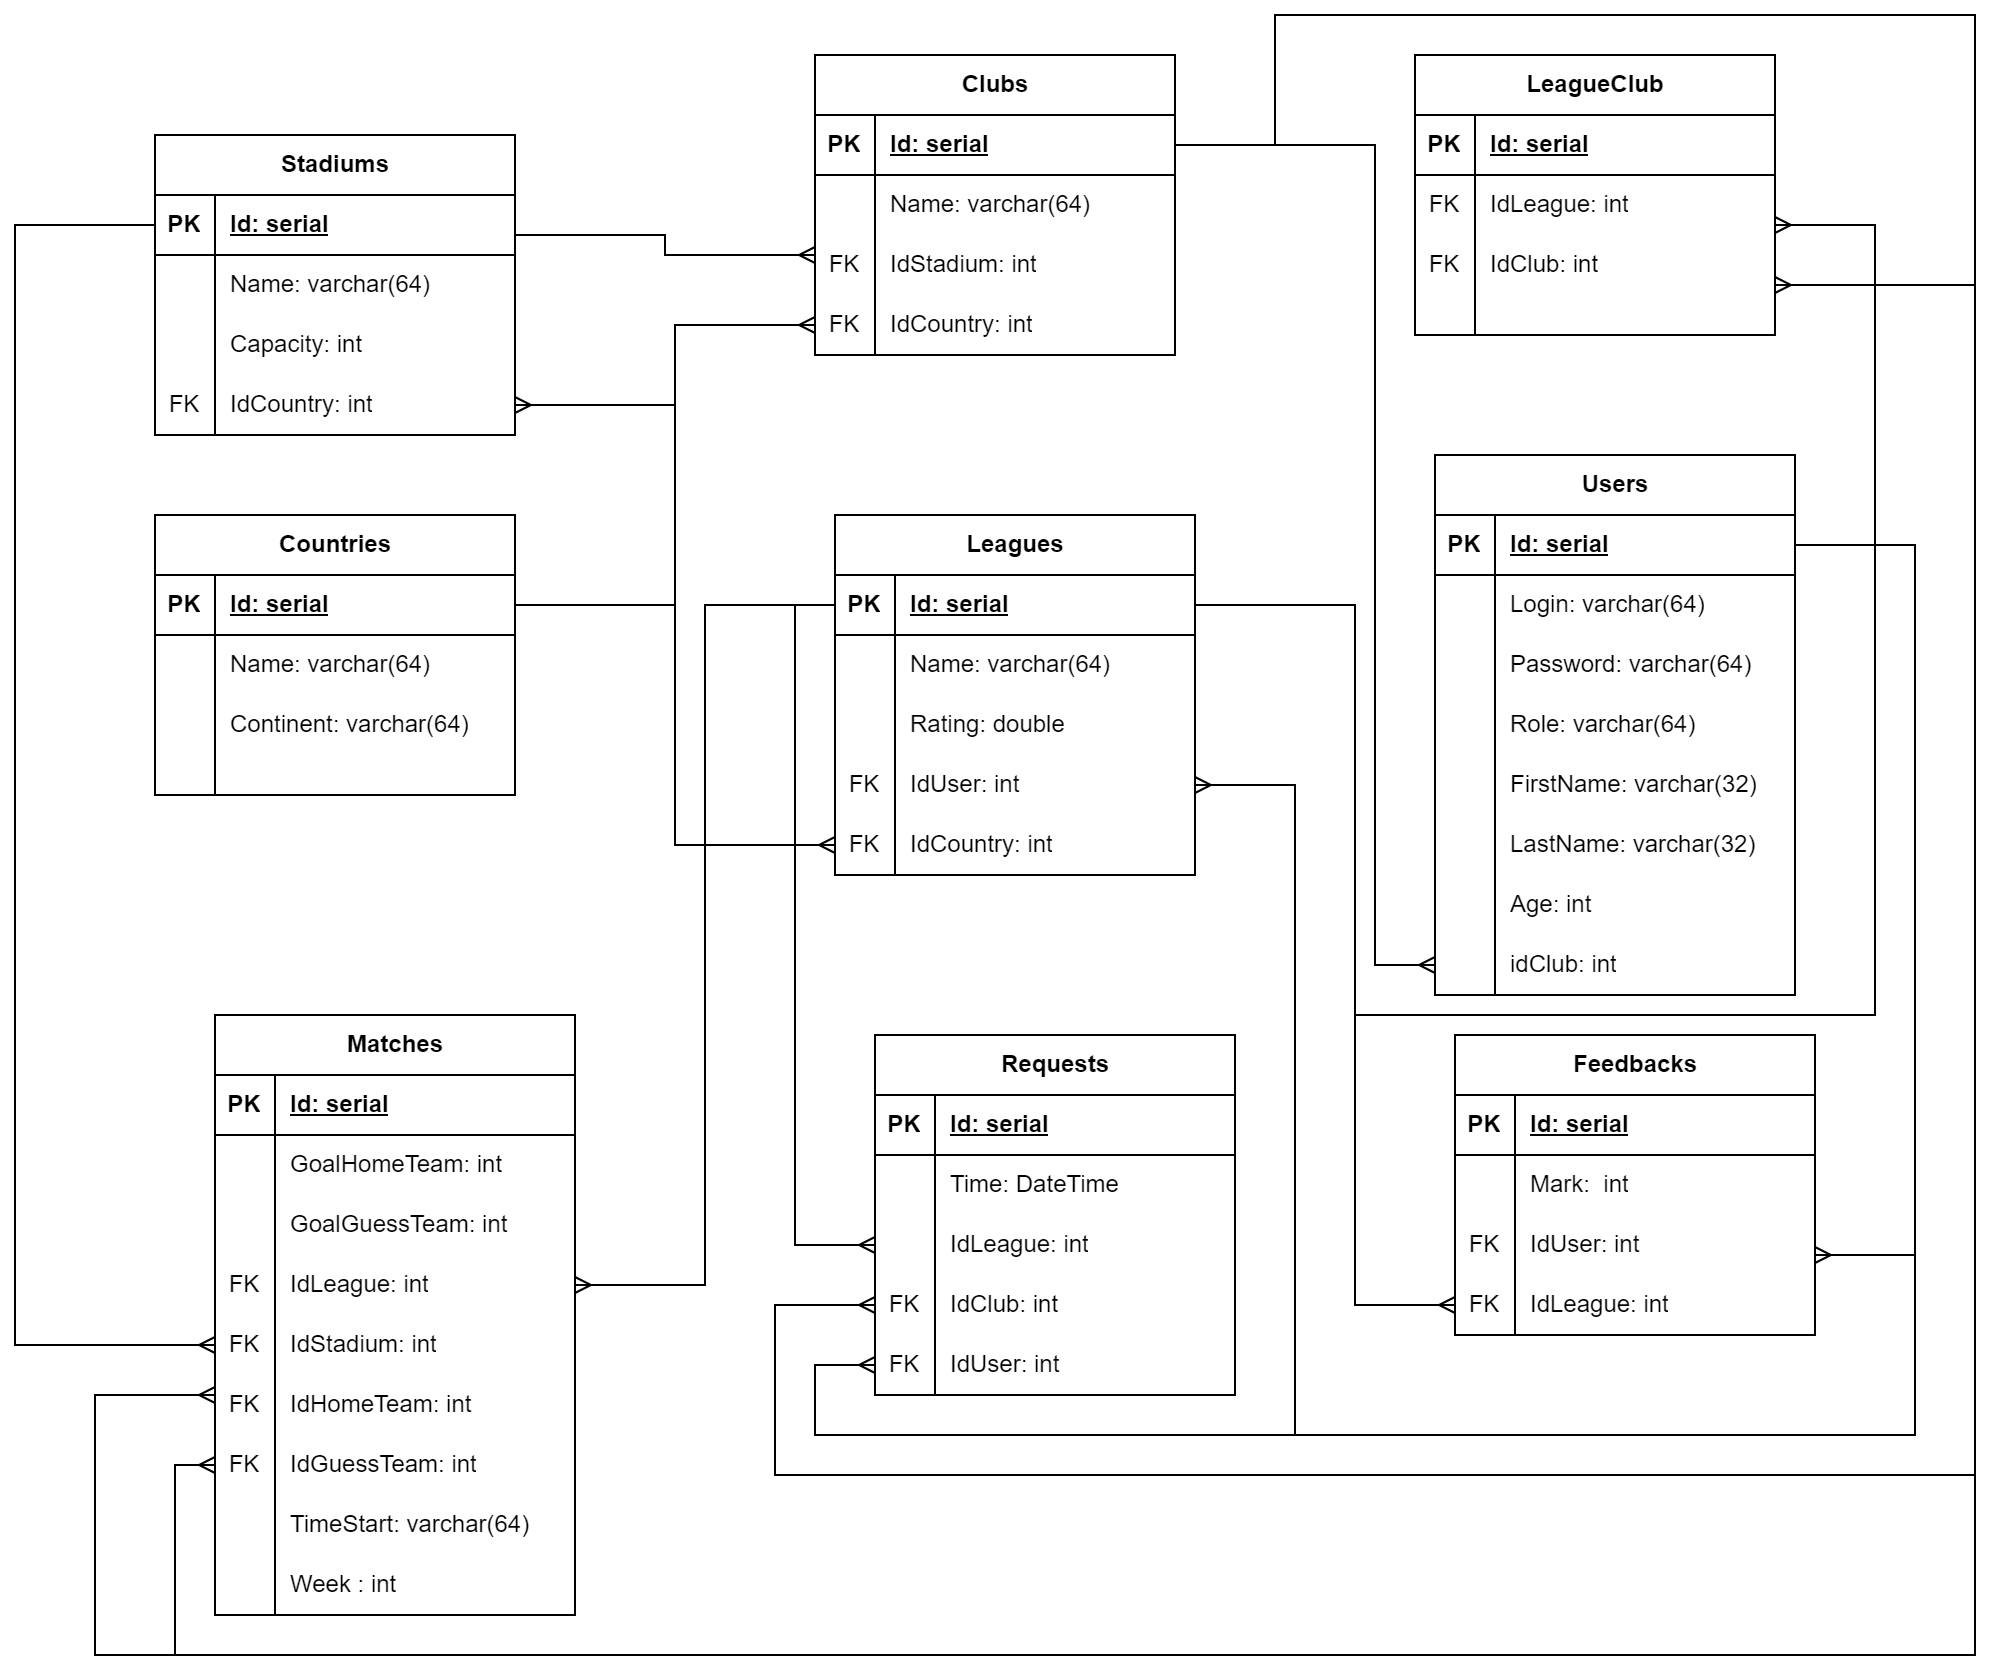
\includegraphics[height=0.5\textheight]{img/ERD.png}
	\caption{ER-диаграмма базы данных}
	\label{img:ERD}
\end{figure}
\clearpage
\subsection{Проектирование приложения}
Приложение будет состоять из 3 компонентов, каждый из которых имеет свою задачу.
\begin{enumerate}
	\item Компонент доступа к базе данных (Data Access) --- выполняет запросы к данным, обеспечивает операции CRUD (Create, Read, Update, Delete).
	\item Компонент реазации интерфейса (UI) --- пользовательский интерфейс, обеспечивает взаимодействие с программой.
	\item Компонент бизнес логики (Business Logic) --- обрабатывает бизнес правила, управляет данными и обрабатывает исключения.
\end{enumerate}

\subsection{Ролевая модель}
В базе данных для каждой группы пользователей, выделенных выше была создана роль:
\begin{itemize}
	\item гость имеет право просмотр всех таблиц, кроме таблиц users, requests, добавления в таблицы users, feedbacks;
	\item футболист имеет право просмотр всех таблиц, кроме таблицы users, добавления в таблицы feedbacks, requests;
	\item тренер имеет право просмотр всех таблиц, кроме таблицы users, добавления в таблицу feedbacks, requests, clubs, удаления в таблице reuquests, clubs, изменения в таблице users;
	\item судья имеет право просмотр всех таблиц, кроме таблицы users, добавления в таблиц leagues, feedbacks, удаления в таблице requests;
	\item администратор имеет право просмор всех таблиц, добавления, изменения, удаление во все таблиы.
\end{itemize}

\subsection{Триггер}

Триггер --- это функция, которая автоматически вызывается после действия (insert, update, delete) над определенной таблицей \cite{light-model}. 

Когда пользователь оставляет свои отзывы, необходимо пересчитать рейтинг турнира.
При добавлении пользовательского отзыва нужно обновить значение поля <<rating>> в таблице турнира. Для процесса перерасчета рейтинга было бы удобно создать триггер, который обновляет поля рейтинга автоматически при добавлении отзыва.

На рисунке \ref{img:trigger} приведена схема триггера для автоматически перерасчета рейтинга турнира.

\begin{figure}[h]
	\centering
	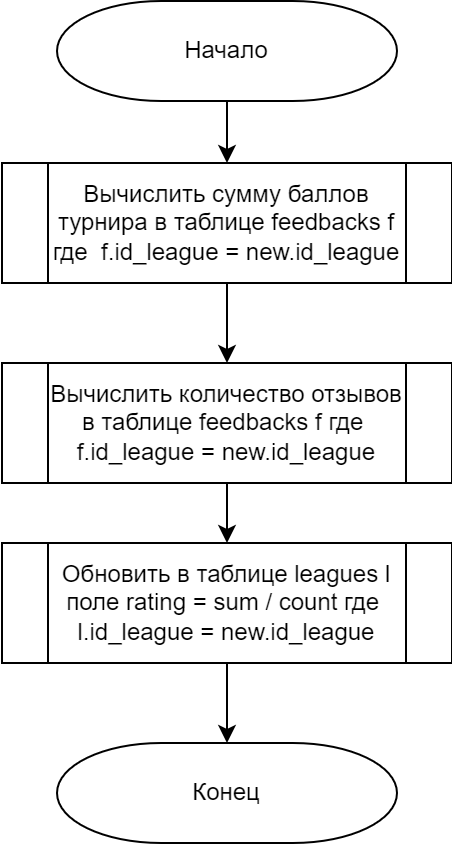
\includegraphics[height=0.4\textheight]{img/trigger.png}
	\caption{Триггер для автоматически перерасчета рейтинга турнира}
	\label{img:trigger}
\end{figure}

\subsection{Алгоритм составления расписания турнира}

Условием организации футбольного турнира является то, что количество участвующих команд должно быть четным.

Турнирное расписание матчей для набора команд , удовлетворяющее приведенному ниже набору ограничений:
\begin{itemize}
	\item ни одна команда не должна играть 2 матча подряд в одной неделе;
	\item каждая команда должна была играть ровно 2 матча со всеми остальными командами. Второй матч состоится после встречи всех оставшихся команд;
	\item интервал между двумя матчами равен неделе.
\end{itemize}

На рисунке \ref{img:schedule} приведена схема алгоритма составления расписания турнира.

\begin{figure}[h]
	\centering
	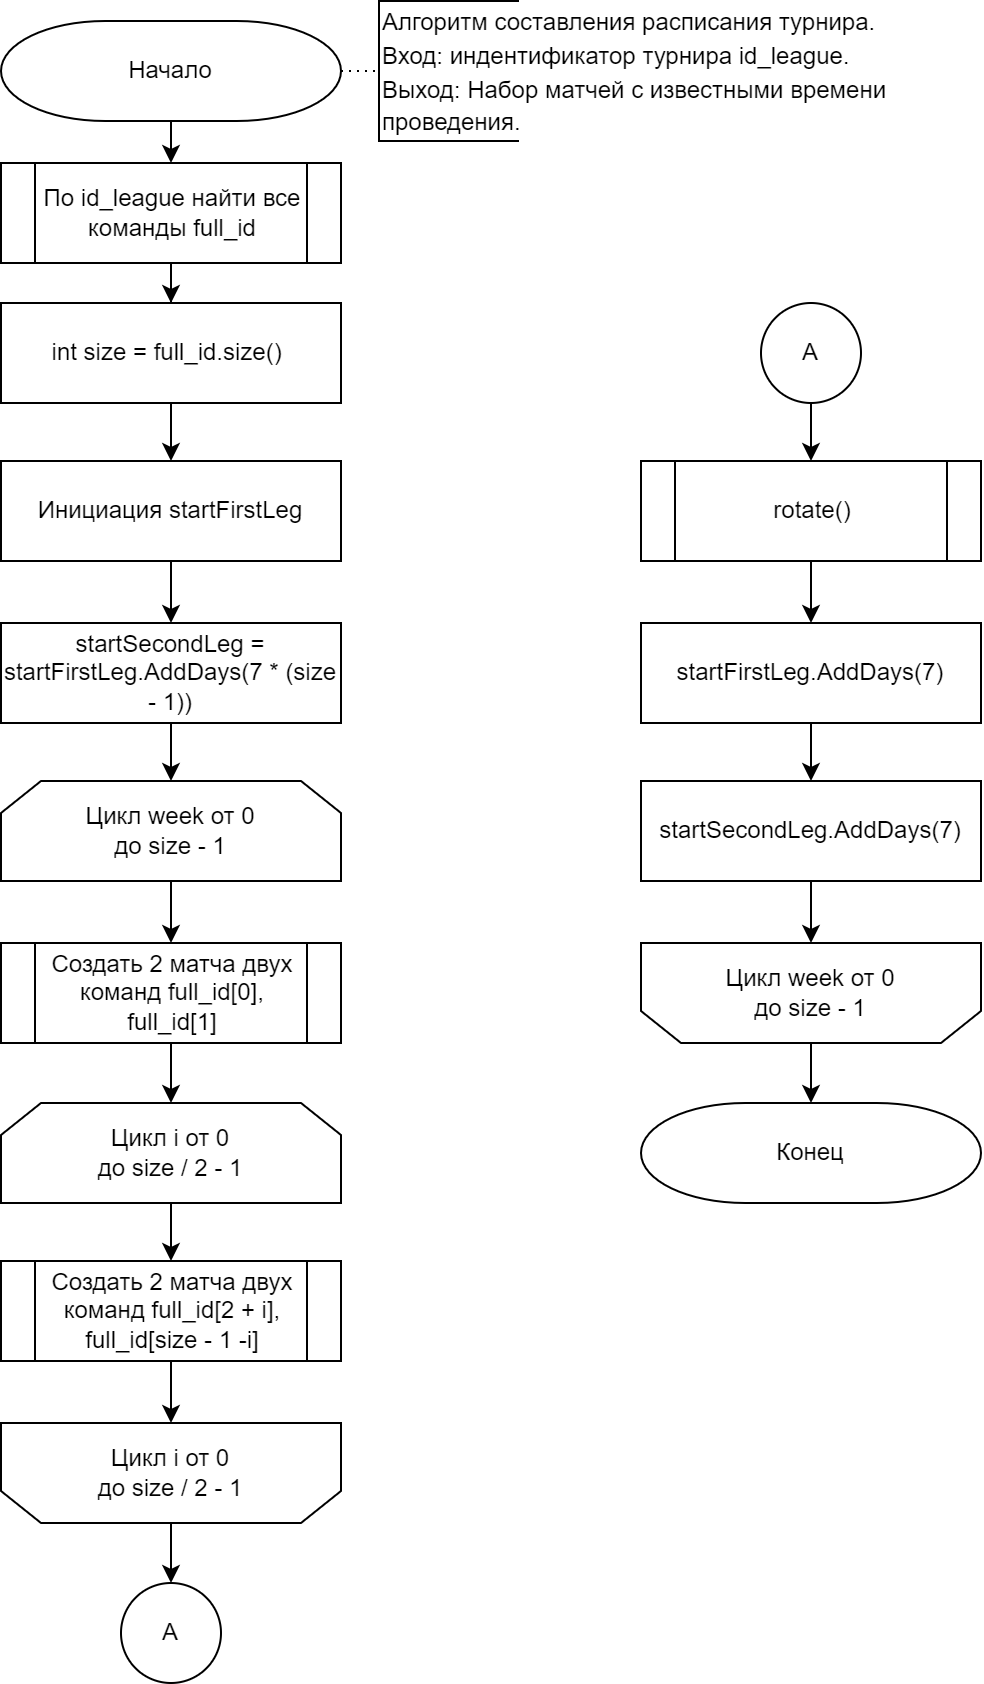
\includegraphics[height=0.45\textheight]{img/schedule.png}
	\caption{Алгоритм составления расписания турнира}
	\label{img:schedule}
\end{figure}
\clearpage

\subsection*{Вывод}
Были приведено проектирование базы данных и проектирование приложения.
Также был спроектирован триггер, осуществляющие автоматически пересчитывать рейтинга турнира при добавлении новых оценок.